% !TeX root = ../../libro.tex
% !TeX encoding = utf8

\chapter{Introducción}

% TODO -- estructura que le quiero dar al trabajo
% 1. Introduccion
% 1. Hablar del problema de retrieval de imagenes, y por qué este problema es relevante
% 1. Hablar del dataset que hemos empleado y de otros datasets que hemos considerado
% 1. Explicar el triplet loss, ventajas que se plantean en el paper de referencia
% 1. Desarrollo de Software
%     1. Explicar las herramientas usadas (entornos de python, librerias principales)
%     2. Explicar github CI CD
%     3. Explicar como accedemos al servidor
%     4. Explicar toda la estructura del codigo, patrones de diseños, sacarme partido aqui que es donde mas fuerte estoy
% 1. Hablar de la aproximacion al problema, iterativa, usando MNIST, LFW, luego CACD + FG-Net
%     - Esto se puede meter en algo asi como planificacion. Lo justifico diciendo que habia mucho codigo nuevo que implementar, y que para iterar de forma rapida iba resolviendo problemas cada vez mas complejos y mas pesados en lo que tamaño de datset se refiere
% 1. Analisis de los malos resultados
% 1. Proponer mejoras a estos problemas

% TODO -- tomar de referencia la guia de Pablo Mesejo: https://drive.google.com/drive/folders/1BGI7zUp0kiZ6ufCH1UlhzvcFPdZ5NFWN
% A partir de esta, importante:

% 1. Dar prioridad al resumen, introduccion (descripcion del problema, motivacion, objetivos) y las conclusiones (**"deben estar perfectas"**)
% 2. Introducir una figura de SCOPUS

Las \textbf{ideas principales} de este trabajo son dos. En primer lugar, resolver un problema de \textbf{reconocimiento facial invariante a cambios en la edad}, por sus siglas en inglés, \entrecomillado{AIFR}. Dentro de este problema, nos centraremos en resolver una tarea de \textbf{retrieval}. En segundo lugar, introducir una nueva técnica de aprendizaje automático, que busca \textbf{solucionar los principales problemas que plantea el uso de la función de pérdida \entrecomillado{triplet loss}} \footnote{Esta nueva técnica se introduce en \cite{matematicas:principal}}. Introduce una forma de generar los \textit{batches} de triples de forma \textit{online}. Evitando así tener un paso separado en el ciclo de entrenamiento, dedicado únicamente a volver a generar de forma \textit{offline} nuevos \textit{batches} de triples. Y de paso, se consigue normalizar la dificultad que suponen estos conjuntos de triples.

Esta situación plantea una serie de \textbf{problemas}:

\begin{itemize}
    \item La nueva técnica de aprendizaje automático se plantea en un \textbf{ambiente completamente distinto} al de \textit{AIFR}, en concreto, en el ámbito de re-identificación de personas.
        \begin{itemize}
            \item En este último, se trabaja normalmente con imágenes de cuerpo completo, y momentos del tiempo muy cercanos. Los problemas que aquí se buscan tratar son, entre otros, seguir identificando con la misma identidad a una persona que ha desaparecido momentáneamente de la escena. Mientras que los problemas principales en \textit{AIFR} son otros (y se detallarán en \customref{ich:descrp_problema})
            \todo{Encontrar un paper que hable de los problemas que tiene re-id. Mirar las introducciones en busca de esto}
            \item Por tanto, no disponemos de literatura en la que se expongan resultados obtenidos de aplicar estas técnicas a nuestro ámbito de trabajo
        \end{itemize}
    \item Esta técnica cambia fundamentalmente la forma de generar \textit{batches} de datos. Y por tanto, modifica en esencia muchas partes primarias del proceso de aprendizaje. Por ejemplo, el ciclo de entrenamiento, el cálculo de métricas durante el entrenamiento, el acceso a los datos. Es por este motivo que hemos tenido que realizar \textbf{implementaciones personalizadas de casi todos estos elementos}, sin poder hacer uso de la mayoría de implementaciones que ofrecen las librerías de aprendizaje automático. Esto supone un \textbf{consumo de tiempo mayor}, teniendo en cuenta que hay que prestar \textbf{especial atención a la optimización y validación} mediante \textit{tests} de estos nuevos módulos
    \item Como comentaremos en \customref{ich:conclusiones}, este trabajo \textbf{no ha dado buenos resultados en la práctica}, comparado con otras técnicas más establecidas en el ámbito del \textit{AIFR}. Sin literatura que aplique nuestras nuevas técnicas en nuestro ámbito, tenemos que \textbf{basarnos en todo el trabajo realizado para estudiar el por qué} de este mal comportamiento.
\end{itemize}

Por otro lado, el ámbito de aplicación de un modelo capaz de reconocer caras independientemente de cambios de edad es amplio, destacando el ámbito de la informática forense. Es muy interesante disponer de un modelo que reconozca caras de sospechosos que llevan en busca un tiempo, o de personas que han desaparecido hace un tiempo y de la que no se disponen imágenes actuales. También para verificar fotografías en documentos de identidad, como pasaportes \cite{informatica:tecnica_sintesis_aifr}.

\section{Descripción del problema} \label{ich:descrp_problema}

Como ya se ha comentado, trabajaremos un problema de reconocimiento facial invariante a la edad (\textit{AIFR}, de sus singlas en inglés \entrecomillado{Age-Invariant Face Recognition}), con la idea principal de introducir una variación sobre la función de pérdida \textit{Triplet Loss} para poder generar \textit{batches} de datos de forma \textit{online}. En esta sección nos centraremos en presentar el problema \textit{AIFR}, la nueva técnica de cómputo de la función de pérdida será explorada en profundidad en \customref{isec:triplet_loss}.

El \textbf{problema de reconocimiento facial invariante a la edad} es el siguiente: dada una imagen de una persona a una cierta edad, ser capaces de discriminar entre imágenes de otras personas y de la persona de la que disponemos la primera imagen, teniendo en cuenta cambios significativos en las edades de las personas que aparecen en las imágenes.

Este problema se puede aún especificar más, en las siguientes tareas:

\begin{itemize}
    \item \textbf{\textit{Retrieval}} o búsqueda: dada una imagen de una persona y una base de datos de imágenes, devolver un número específico de imágenes de la misma persona

        \begin{itemize}
            \item Esta es la tarea que se intenta resolver en el presente trabajo
            \item Un escenario para esta tarea es, por ejemplo, tras la desaparición de una persona, tomar imágenes de distintas bases de datos policiales y estudiar las 100 imágenes con mayor potencial de apuntar a la persona indicada
            \item A la acción de aportar una imagen, una base de datos, y tomar las $N$ imágenes que son más probables de coincidir en la identidad de la persona de la primera imagen, la llamaremos \textbf{consulta} o \textbf{\textit{query}}
        \end{itemize}

    \item Verificación: dada dos imágenes, el modelo debe decidir si se tratan de la misma persona o no.
        \begin{itemize}
            \item Un escenario es, por ejemplo, comprobar la imagen del pasaporte y la imagen obtenida de las cámaras de los puestos de control de acceso automático
        \end{itemize}

    \item Clasificación: habiendo entrenado sobre un conjunto de individuos prefijado, dada una imagen de entrada, identificar al individuo que aparece en dicha imagen como alguno de aquellos vistos durante el entrenamiento
        \begin{itemize}
            \item Esto fuerza a que solo podamos trabajar con un número prefijado de personas, y no con personas arbitrarias que nunca hayamos visto antes. Esta restricción hace que sea la tarea menos interesante (y quizás, la más sencilla de resolver), y por tanto, es inusual encontrar trabajos que usen técnicas relacionadas con las que más adelante presentado para intentar resolver estos problemas
        \end{itemize}
\end{itemize}

Por lo tanto, realmente nuestra tarea es la de realizar \textit{retrieval} de imágenes faciales invariantes a cambios en la edad. Sin embargo, en adelante, salvo que induzca a confusión, nos referiremos a esta tarea simplemente como \textit{AIFR}, sin especificar que estamos realizando concretamente \textit{retrieval} y no otras de las tareas que ya hemos detallado

Este problema tiene, además de los problemas comunes de la visión por computador, las siguientes \textbf{dificultades específicas} \cite{informatica:challenges_retrieval}:

\begin{itemize}
    \item \textbf{Invarianzas}: en nuestro problema esto es especialmente relevante. Al trabajar con imágenes tomadas en, potencialmente, instantes de tiempo muy variados, las características de la imagen pueden variar considerablemente.
        \begin{itemize}
            \item Pensemos, por ejemplo, en fotografías pasadas que fueron tomadas en blanco y negro, en contraste con fotografías más actuales en color
            \item O problemas más relevantes (pues el anterior es fácil de solventar), como cambios relevantes en características de la cámara con la que se toman las fotografías
        \end{itemize}
    \item \textbf{Distractores}: nuestro modelo se debe centrar en estudiar las caras que aparezcan en la imagen, ignorando otros elementos, como los que puedan aparecer en el fondo de las imágenes
    \item \textbf{Eficiencia}: a la hora de que nuestro modelo reciba una \textit{query}, desconocemos el tamaño de la base de datos sobre la que tenemos que operar. Por tanto, nuestro modelo deberá ser eficiente para poder trabajar con grandes bases de datos sin que el tiempo de respuesta se vea gravemente afectado
    \item Problemas asociados al bold{envejecimiento}: cómo varía la cara con el paso de los años es un proceso muy complejo. Algunos de los factores que afectan a este envejecimiento \cite{informatica:tecnica_sintesis_aifr} son:
        \begin{itemize}
            \item Factores intrínsecos como la genética o la etnia
            \item Factores extrínsecos como el ambiente o los hábitos de vida
        \end{itemize}
    Además, algunas características de la cara cambian drásticamente con el paso de los años. Por ejemplo, la textura (pensar por ejemplo en la aparición de arrugas, lunares, vello, \ldots), cambios en la forma de la cara (por ejemplo, por un cambio en el peso corporal)

\item Tenemos que trabajar con \textbf{identidades que nunca hemos visto} en nuestros datos de entrenamiento. En otras tareas, como por ejemplo la de clasificación de objetos cotidianos, también ocurre esto (por ejemplo, tenemos imágenes de coches que nunca ha visto previamente el modelo). Sin embargo la diferencia radica en que, en nuestro problema, el modelo debe saber identificar identidades, mientras que en el segundo caso, el modelo debe saber identificar categorías. Siguiendo con esta analogía, sería como pedirle al modelo clasificador que, dados dos tipos de objetos que nunca ha visto (por ejemplo, aviones), sepa asignarles la misma categoría

\item Aunque desarrollemos esto más tarde en \customref{isec:base_datos_usada}, los \textbf{\textit{datasets} de \textit{AIFR} son escasos y presentan problemas} \cite{informatica:tecnica_sintesis_aifr}. Algunas de estas bases de datos son muy pequeñas. Otras, son de un tamaño más grande, pero presentan mucha menos variabilidad en los rangos de edad. Y por supuesto, muchas de estas bases de datos presentan problemas de representatividad (etnia, sexo).
\end{itemize}

\begin{figure}[H]
\centering
    \begin{subfigure}{0.5\textwidth}
        \centering
        \includegraphics[width=0.6\linewidth]{informatica/messi_niño}
        \caption{Edad temprana}
        \label{img:messi_pequeño}
    \end{subfigure}%
    \begin{subfigure}{.5\textwidth}
        \centering
        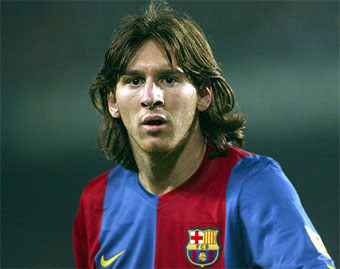
\includegraphics[width=0.8\linewidth]{informatica/messi_joven}
        \caption{Edad joven}
    \end{subfigure}%

    \begin{subfigure}{.5\textwidth}
        \centering
        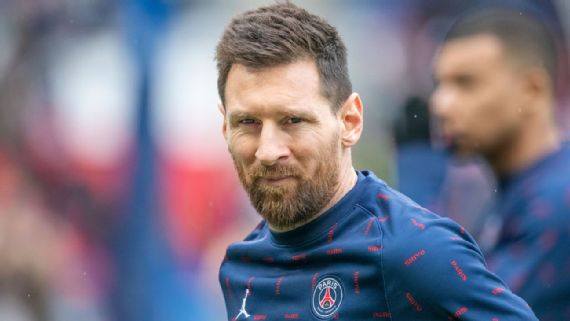
\includegraphics[width=0.8\linewidth]{informatica/messi_adulto}
        \caption{Edad adulta}
        \label{img:messi_adulto}
    \end{subfigure}%
    \begin{subfigure}{.5\textwidth}
        \centering
        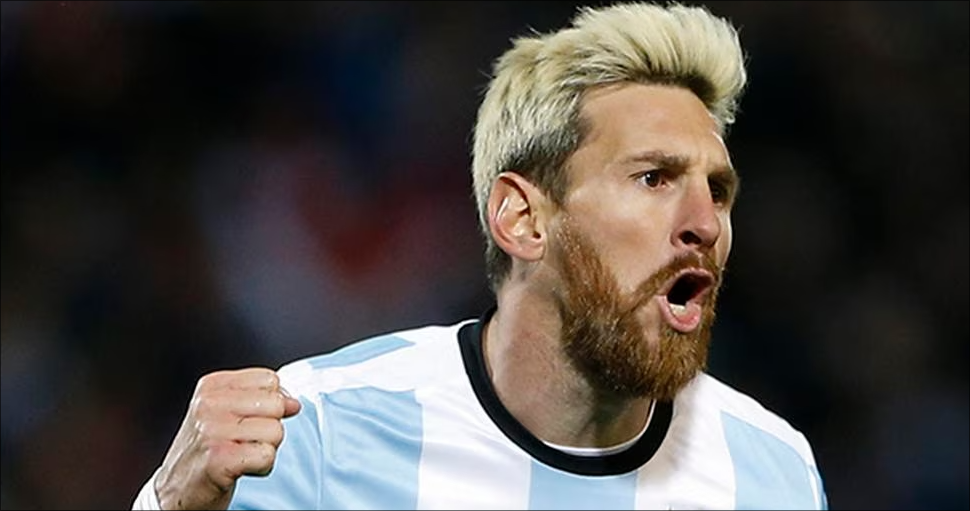
\includegraphics[width=0.8\linewidth]{informatica/messi_rubio}
        \caption{Otra imágene ne la edad adulta, pocos años después}
    \end{subfigure}

    \caption{Lionel Messi en cuatro momentos distintos de su vida}
    \label{img:messi_cuatro_edades}

\end{figure}

Por poner un ejemplo, fijémonos en \customref{img:messi_cuatro_edades} \footnotemark. Estas cuatro imágenes reflejan perfectamente los problemas que hemos planteado previamente. Por ejemplo, en la fotografía \ref{img:messi_adulto} podemos ver que, en el fondo de la imagen, aparece otro jugador, y nuestro modelo podría distraerse por este hecho. La imagen en la que aparece siendo más pequeño, \ref{img:messi_pequeño}, es de una calidad mucho menor que el resto de imágenes. No ha desarrollado todavía rasgos faciales muy característicos. La variabilidad en el estilo de pelo es total. Se puede apreciar perfectamente como el paso de los años va modificando los rasgos de la cara. Y todo esto sin comentar problemas comunes y bien conocidos en la visión por computador, como por ejemplo, cambios en la pose, iluminación, \ldots
\footnotetext{Imágenes extraídas de \url{https://tinyurl.com/2x4fkxjx}, \url{https://tinyurl.com/y4ubnz3v}, \url{https://tinyurl.com/ywek233h} y \url{https://tinyurl.com/yqrf78w8}}

Y aunque más tarde desarrollemos en profundidad el uso de \textit{triplet loss} (\customref{isec:triplet_loss}), conviene hacer ahora unos pequeños apuntes sobre esta técnica. Para empezar, el uso de esta función de pérdida ya nos indica que, de una forma u otra, nuestra solución al problema va a fundamentarse en el cómputo de un \textit{embedding}.

Por tanto, usando dicho fundamento, podríamos haber resuelto también alguno de los otros problemas que ya hemos mencionado, por ejemplo, el de verificación. Sin embargo, para acotar el alcance de este trabajo, hemos decidido centrarnos en \textit{retrieval}.

Además, por cómo hemos diseñado el código (basado en adaptadores, como explicamos en \customref{ich:implementacion}), la adaptación del modelo a una nueva tarea es inmediato, y en teoría, si el modelo inicial es competente, el modelo adaptado también debería serlo.

Y para finalizar, comentaremos los \textbf{dos enfoques principales usados para resolver problemas de \textit{AIFR}}:

\begin{enumerate}
    \item El primer enfoque es aplicar modelos generativos adversarios (\textit{GAN}). Por ejemplo, el \textit{Age Invariant Model} o \textit{AIM} propuesto en \cite{informatica:tecnica_sintesis_aifr}.
    \item El segundo enfoque es directamente trabajar sobre una base de datos que presente la suficiente variabilidad en la edad de los individuos, y desarrollar un modelo que realice nuestra tarea. Este enfoque casi siempre pasa por computar un \textit{embedding}. Este será el enfoque que sigamos.
\end{enumerate}

\section{Descripción de la base de datos usada} \label{isec:base_datos_usada}

Como se comentará en \customref{isec:planificacion}, teniendo en cuenta que íbamos a tener que realizar un gran número de implementaciones, decidimos iterar sobre varias bases de datos.

La \textbf{primera base de datos} que consideramos es la más que conocida \entrecomillado{MNIST} \cite{informatica:mnist}. Esta base de datos se compone de 70000 imágenes $28 \times 28$ de dígitos, del 0 al 9, escritos a mano. No tiene ningún interés para el trabajo que vamos a realizar. Sin embargo, escogemos esta base de datos como punto de partida por:

\begin{itemize}
    \item Es una base de datos muy pequeña, por lo que nuestras implementaciones no tendrán ningún tipo de problemas de rendimiento
    \item Es una base de datos muy sencilla, no tenemos que preocuparnos de procesar las imágenes de ninguna forma
    \item No tenemos que realizar ninguna implementación para trabajar con ella, puesto que podemos usar el paquete \lstinline{torchvision}, que se encarga de la descarga del conjunto de datos y su disposición en un objeto de tipo \lstinline{torch.utils.data.Dataset}
\end{itemize}

\section{Descripción de los objetivos}
\todo{Esta sección no me convence nada, volver a ella cuando haya desarrollado más texto}

Por todo esto, los objetivos del presente trabajo son los siguientes:

\begin{enumerate}
    \item Realizar una revisión del estado del arte en el ámbito del \textit{AIFR}
    \item Implementar todos los módulos necesarios para poder aplicar técnicas \textit{online} de cómputo del \textit{triplet loss}
    \item Realizar un estudio de los \textit{datasets} disponibles
    \item Comparar los resultados obtenidos con otros trabajos del mismo ámbito
\end{enumerate}

\section{Planificación} \label{isec:planificacion}

Tras un estudio inicial de los \textit{frameworks} de aprendizaje automático existentes, nos damos cuenta de que no hay implementaciones para las técnicas sobre las que queremos estudiar. Esto supone que deberemos dedicar un gran esfuerzo al diseño, implementación, optimización y validación de módulos de código. Por tanto, decidimos realizar un desarrollo en varias etapas, iterando sobre distintas bases de datos, de menor complejidad (estructura de los datos, facilidad de trabajo con ellos, tamaño) e interés, hasta los datos más complejos y relevantes para nuestro estudio.

Esto ha permitido poder centrarnos en el desarrollo de los módulos, sin preocuparnos de los problemas que podrían introducir distintas bases de datos. Una vez realizada una implementación inicial junto con su validación a partir de una base sólida de \textit{tests}, se itera sobre bases de datos más complejas, en busca de analizar posibles problemas de rendimiento. Y así es como acaba ocurriendo, como plasmamos en \customref{isec:optimizacion_codigo}.

Una vez analizados y resuelto los puntos débiles en temas de rendimiento (evitando así realizar optimizaciones prematuras e irrelevantes que ralentizasen el desarrollo de código), pasamos a tratar con las bases de datos que realmente nos interesan. Así, en este punto, tenemos prácticamente toda la base de código desarrollada, pudiendo centrarnos únicamente en la experimentación.

\todo{Todavía le faltan partes}
